\documentclass[conference]{IEEEtran}
\IEEEoverridecommandlockouts
% The preceding line is only needed to identify funding in the first footnote. If that is unneeded, please comment it out.
\usepackage{cite}
\usepackage{amsmath,amssymb,amsfonts}
\usepackage{algorithmic}
\usepackage{graphicx}
\usepackage{textcomp}
     % for random text
\usepackage{xcolor}
\def\BibTeX{{\rm B\kern-.05em{\sc i\kern-.025em b}\kern-.08em
    T\kern-.1667em\lower.7ex\hbox{E}\kern-.125emX}}
\begin{document}

\title{Localization with activity recognition and particle filter\\}

\author{
\IEEEauthorblockN{1\textsuperscript{st} Bergauer Philipp}
\IEEEauthorblockA{\textit{TU Graz} \\
Graz, Austria\\
philipp.bergauer@student.tugraz.at
}
\and
\IEEEauthorblockN{2\textsuperscript{nd} Halici {\"O}mer Faruk}
\IEEEauthorblockA{\textit{TU Graz} \\
Graz, Austria\\
halici@student.tugraz.at}
}

\maketitle

\begin{abstract}
The Activity Recognition keeps track if the user is moving or staying in the same Position. It is able to classify if the user is standing, sitting or walking. The localization App can be used calculate where the user is in the 16 building of the Inffeldgasse Graz. Because an Particle Filter was used it is only able to get an accurate Position of the user if the user walked around enough.
\end{abstract}

\section{Introduction}
To keep track of the Activity of the user the Acceleration sensor of the Android phone was used. After a view values of the Acceleration sensor the samples were classified with an k Nearest Neighbor(k-NN) Algorithm. The Algorithm is able to classify the three activities sitting, standing and walking. For Localization the Activity recognition was used to keep track if the user is walking or not walking. With this Information an Particle Filter was used to classify were the user is if he walks arround. The Particle Filter didn't use any additional sensor Informations so it does not have your exact   position when the app is started. The user needs to walk arround a little bit and after that the Particle Filter notice where the Person is in the 16 Inffeldgasse building.
The Localization was splited into two parts, the first part was an Activity recognition and the second part was the localization Algorithm with the Particle Filter. The Activity recognition was implemented with an k-Nearest Neighbor(k-NN) algorithm. It was used to classify if the user is moving or not. 

\section{Activity recognition}
The mobile phone has many sensors. Some of them can be used to track the activity of a person.  After collecting sensor data the patterns in the data can be retrieved and can be used to classify between activities e.g jogging,running, walking.
\subsection{Tensorflow approach for Convolutional Neural Network}
Our first approach was to use the popular tensorflow framework from Google. The idea was to train and write the cody in python and export a tensorflow model which can be used by our mobile phone. The trainingsdata was taken from the Wireless Sensor Data Mining group\cite{b1}. We decided to use a CNN network because it can be used to analyze interesting fatures in the data set. The error rate for the trainings data was very low. Only 15 \% were missclassified. The export to the android device worked too but in the end it did not work as accurate enough. The problem was that our dataset and our own sensor data generated from our mobile phones were to different so the model missclassified most of the activites wrong. Afterwards we tried to train our CNN with our own trainingsset. It got better but it never worked in practice. We have three theories why it did not work after all. First overfitting the model. Second a bug when exporting the model. We stored it as a pb file and labeled input and output falsely. Third and last theory would be that the model was designed wrong. After days of debugging and fixing some errors we came to the conclusion to go along with the K-NN approach\cite{b2}.
\subsection{K-NN approach}
First of all the K-NN algorithm is one of the simplest and most used classification algorithms. The classification of an object/class uses the majority vote of its neighbours. There are many decisions to be made before implementing the K-NN. First of all which K should we take. The K stands for the number of neighbours to be taken in account. It should be an odd number. In our case it was 21. The calculation of the distance is another point to think about. We decided to use the euclidean distance for our K-NN. The formula of the euclidean distance:
\begin{equation}
D(w_i,v_i) = \sqrt{\sum{(w_i - v_i)^2}}
\end{equation}
The euclidean distance is easy to program and is very efficient. We measured the time for one classification of the samples and it was less than 50 ms. The measurement started after collecting all necessary data.
\begin{figure}
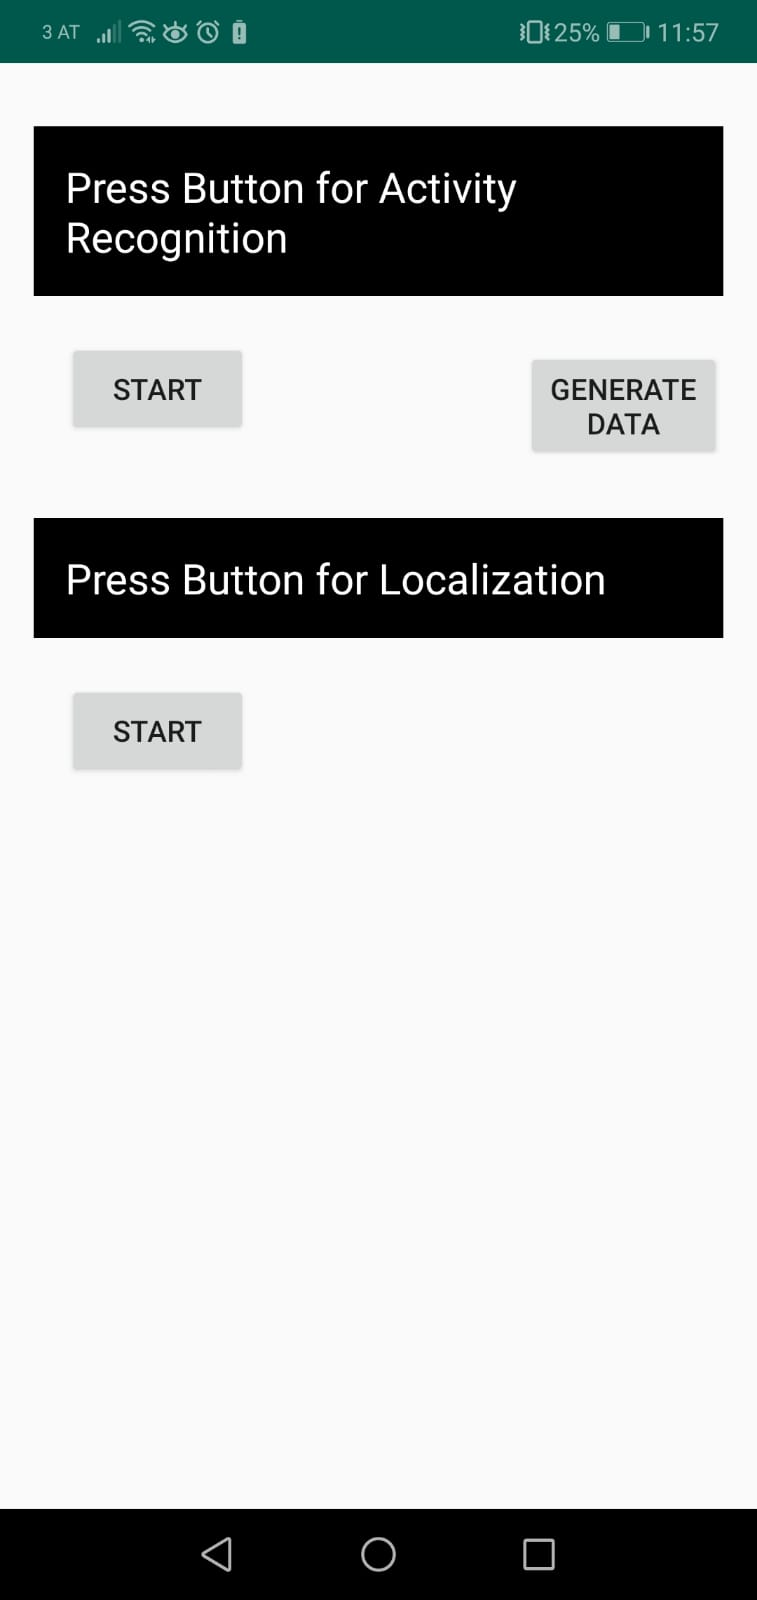
\includegraphics[height = 7.5cm,width = 5cm]{Images/MainActivity.jpeg}
\centering
\caption{MainMenuActivity of the application}
\label{fig:mainmenuactivity}
\end{figure}
\subsection{Feature extraction}
Afterwards we thought about the features to use for the data set and the window size. We took the same features as for our CNN.The mean for each axis of the accelerometer values, the max peaks in each axis,the min peaks in each axis and the variances of each axis. 
In addition one record contains 20 samples too. The sample rate can be adjusted in android so we took the sampling rate $SENSOR\_DELAY\_FASTEST$. According to its name it should be the fastest one. The windows size are 20 samples. The sampling rate is dependable on the hardware in the mobile phone, so it is hard to give a window for 20 samples in seconds but it should be approximately 50ms. 
\subsection{Data generation}
The reference dataset was  taken with the SensorHandler class. These class takes the samples and writed them in a txt file. In our main activity we can click on the generate data button and generate data for our classificitation as shown in \ref{fig:mainmenuactivity}. It is worth mentioning that we stored our collected trainingsdata in the asset folder so a user only needs the apk to use the activity recognition. The asset folder contains all necessary data for the application.\\ 
With our own dataset and the extracted features we could classify. We differentiated between 3 classes:Walking,Standing and Sitting. It should be explicitly noted that our activity recognition works with the phone in the pocket. 
\subsection{Classifier}
\begin{figure}
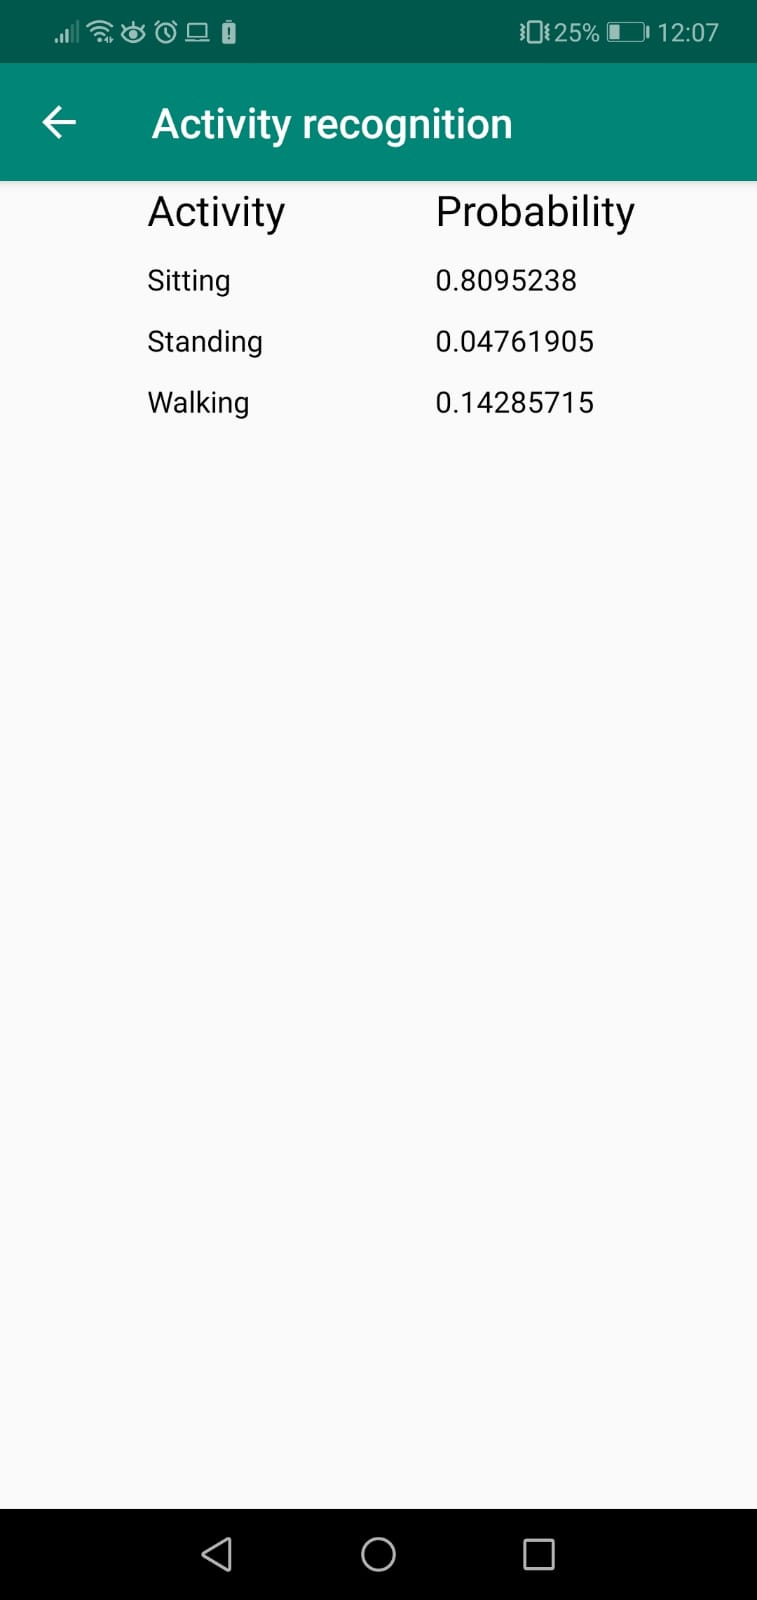
\includegraphics[height = 7.5cm,width = 5cm]{Images/AcitivityRecognition.jpeg}
\centering
\caption{Activityrecognition with accelerometer values }
\label{fig:classifier}
\end{figure}
As seen in figure \ref{fig:classifier} the K-NN algorithm classified sitting right with an accuracy about 80 \%. The classifier is very fast because we use the fastest sampling rate possible. The best classification are walking and standing because the accelerometer values are much apparent to our classifier.

\section{Localization}
The next step was using the activity recognition with accelerometer values to start a localization in a buildung given the map or floorplan of the buildung. The localization should be done with a particle filter. First we want to talk about the parsing through the given floorplan.
\subsection{Floorplan}
For the Paritcle Filter to work, a floorplan of the building where we want to classify the position of the user is needed. So a floorplan of the 16 Inffeldgasse building is taken and edited. All the sections that should not be classified are coloured light grey. Then because the wall has pixel holes a wall finding algorithm was written and the walls were colored red so continues walls were created. In the floor plan was a scale were one rectangle was 5 meters, so that was coloured green and then our programm looked how wide one rectangle was and calculated how many pixels the rectangle was wide, so a factor for meter to pixel was created. After this the orientation sensor (magnetic sensor) has to be calibrated for the building, to have the perfect angle we added an offset of 47 degress to our orientation \cite{b4}. So with this method our programm can be used on every building with very little things to rethink.
 \subsection{Particle Filter}
After everything with the floorplan was done the Particle Filter was implemented. 
\subsubsection{Initilization of particles}
First the Particle Filter executes the init step. In the init step the Particle Filter distributes random 15000 Particle in the sections of the Floorplan that should be taken in account for localization. All this Particles have a weight of $\frac{1}{15000} $ where the 15000 are the number of particles distributed.
\subsubsection{Motion Model}
Then the Motion Model classifies that the user started moving the particles starts moving in the direction and distance the user is moving. For each Particle a bias is added to the movement direction and distance of the user so not all particles are moving to the same direction or have the same distance. This is to work against uncertainness of the movement. The x - Axis is calculated with the following equation.
\begin{equation*}\label{eq:x}
\begin{aligned}
x = paricle_{pos_x} + 0.65f * random.nextDouble() \\ + 0.95f * pixel\_distance * cos(\theta)
\end{aligned}
\end{equation*}
As equation \ref{eq:x} shows the current position with some additions. It is important to mention that the random.nextDouble function returns values between 0 to 1 which are uniformly distributed. 

\begin{equation*}
\label{eq:direction}
\begin{aligned}
\theta = Math.toRadians(direction) +\\ 0.35f * random.nextDouble()
\end{aligned}
\end{equation*}
$\theta$ is the angle taken from the azimuth value as seen in equation \ref{eq:direction}. As mentioned before the azimuth values gets a bias too. First we convert angle to radian and add some noise too.
The same procedure is done to the y - Axis but the main difference is that we weight the x - Axis more than the y - Axis because of the height and width of the floorplan.
\begin{equation*}
\label{eq:y}
\begin{aligned}
y = paricle_{posy} + 0.15f * random.nextDouble() \\ + 0.65f * pixel\_distance * cos(\theta)
\end{aligned}
\end{equation*}
With this in mind we should now think about particles colliding with walls or even going through walls.\\
\subsubsection{Collision}
When an Particle collides with an wall of the floorplan or is in an position which it's not allowed to be there the weight of the particle is set to 0. All particles that are still valid are, get a new weight. The weight is  $\frac{1}{num_particles_survived} $. \\
\subsubsection{Systematic resampling}
The resampling step is the most important and most difficult one to implement. We decided to use the systematic resampling algorithm or sometimes it is called low variance resampling in the literature \cite{b3}. First we generate a probability density function with the weights. The probability density function has N elements. N is the number of particles. After the probability density function we initialize a threshold which we called u. The threshold is incremented in each iteration. We have in sum N iterations. In each iteration we assign a new particle.  We iterate through our probability density function until we reach the threshold. So the new position of the invalid/old particle is an position of an old/valid particle. 
Because of the bias that is added to the movment and orientation in the next step the Particles should be on different positions. The new resampled particles get an weight of $\frac{1}{15000}$. \\
\subsubsection{Estimating position}
For the estimated Position the x and y Position for each Paritcle is taken and an median Filter is applied on the x and y postion. So the estimated position is the middle x and the middle y position of all Particles.
\subsection{Particle Filter in action}
\begin{figure}
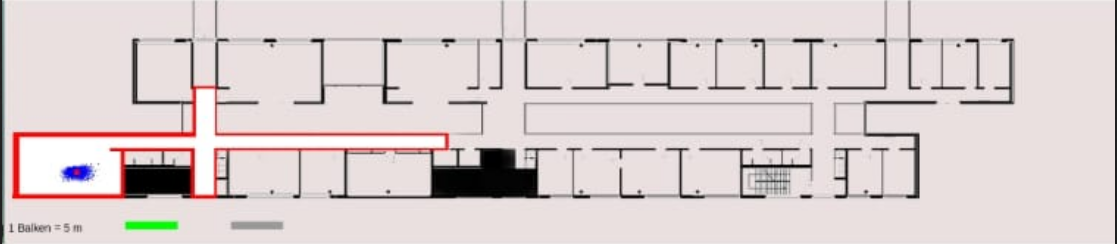
\includegraphics[height = 5cm,width = 10cm]{Images/particle_in_action.png}
\centering
\caption{Application  of the particle filter on the map}
\label{fig:particleinaction}
\end{figure}
After explaining all steps figure \ref{fig:particleinaction} shows how the particle filter performs in real time. The figure in \ref{fig:particleinaction} shows that the close a circle around the position which has the highest possibillity. However the application slowed down because updating the bitmap took too long so we thought about some optimizations.
\subsection{Optimizations for the particle filter and application}
The most important optimization was multithreading. The particle filter is a thread which run one time and dies. So each movement which should call particle filter starts a thread.  In addition the drawing of bitmap is handled by another thread. The draw thread is simultaneously started with the particle filter and does some cleaning of the bitmap and then waits that the particle filter updates all particle positions. When we tested our particle filter sometimes all particles collided with the wall and the application restarted. So to avoid these case set a threshold of living particles and if the amount of valid particles goes under this threshold the initilization step is called again to avoid restarting the app. In addition the particle filter weights x and y axes differently. We came to the conclusion that it makes more sense to weight the axes and the algorithm showed good result with weighting.
\begin{thebibliography}{00}
\bibitem{b1} Jennifer R. Kwapisz, Gary M. Weiss, Samuel A. Moore, ``Activity Recognition using Cell Phone Accelerometers,''  Department of Computer and Information Science  Fordham University  441 East Fordham Road  Bronx, NY 10458.
\bibitem{b2}https://aqibsaeed.github.io/2016-11-04-human-activity-recognition-cnn/
\bibitem{b3}Gerald Steinbauer ,``Advanced Robotics Uncertainty \& Localization II Institute for Software Technology,\\
http://www.ist.tugraz.at/steinbauermediawiki/images/a/aa/Ar19uncertaintyII.pdf, pp 38
\bibitem{b4} https://github.com/osaukh/mobilecomputinglab/blob/master/WS11SensorsandSignals.ipynb
\end{thebibliography}
\vspace{12pt}


\end{document}
